\begin{figure}[h]
	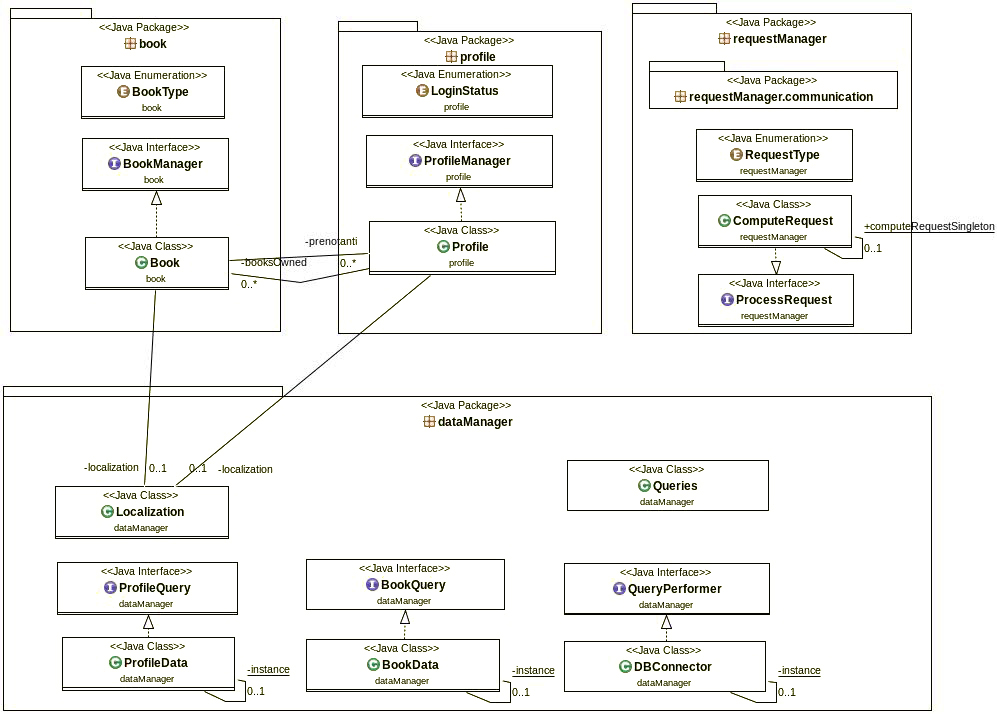
\includegraphics[width=\textwidth]{Immagini/iterazione_1_uml}
	\caption{class diagram}
	\label{fig:xx}
\end{figure}

\begin{figure}[h]
	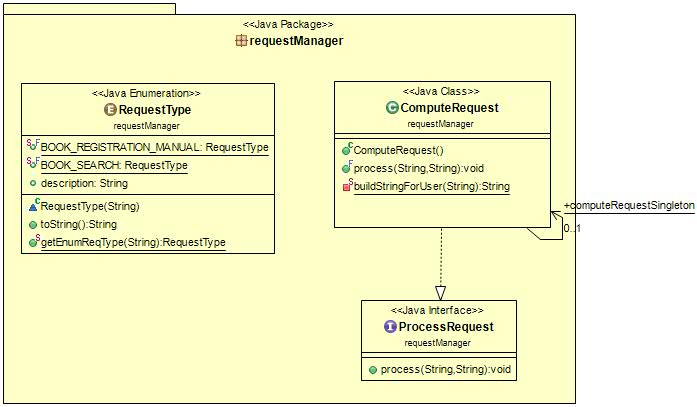
\includegraphics[width=\textwidth]{Immagini/UML_ComputeRequestServer}
	\caption{Diagramma della classe ComputeRequest}
	\label{fig:Diagramma della class ComputeRequest}
\end{figure}

\begin{lstlisting}
public class ComputeRequest implements ProcessRequest{
	~
	public final void process(String msg, String username) {
	// First information is the request type, that 
		is encoded in this way: REQUESTTYPE:...;
		int i = msg.indexOf(";", 0);
		int j = msg.indexOf(":", 0);
		// Convert the String information of the 
		// request type to an enum
		@Nullable RequestType requestType = RequestType.
		getEnumReqType(msg.substring(0, i).substring(j+1));

		if(requestType == null) {
		// In this case, in the request, ther's 
		// a wrong encoded request type
		Communication.getInstance().send(username,
		"requestType:" + 10000 + ";result:KO_RequestType");
		return;
		}

		switch(requestType) {
			case BOOK_REGISTRATION_MANUAL:
				Book b = new Book(msg.substring(i + 1));
				b.setActualOwnerUsername(username);
				b.setISBN("null");

				boolean result = b.insert();
				Communication.getInstance().send(username,
				"requestType:0;result:" + (result?1:0) + 
				";BCID:" + b.getBCID());
				break;
				
			case BOOK_SEARCH:
				~
				if(type.equals("TITLE")) {
					books = BookData.searchBookByTitle(title);
				} else if (type.equals("AUTHOR")) {
				books = BookData.searchBookByAuthor(author);
				} else {
				books = BookData.searchBook(title, author);
				}
				~
				Communication.getInstance().send(username, 
				"requestType:8;result:" 
				+ 1 + ";Books:" + jsonResponse);
				break;
				
				~
		}
	}
}
\end{lstlisting}
